\documentclass[10pt]{article}

\usepackage{amsmath}
\usepackage{amssymb}
\usepackage{array}
\usepackage{tabu}
\usepackage{lmodern}
\usepackage{graphicx}
\usepackage[space]{grffile}
\usepackage{subfigure}
\usepackage{longtable}
\usepackage{multirow}
\usepackage[margin=1.0in]{geometry}
\renewcommand{\baselinestretch}{2.0}

%\usepackage[font=small,labelfont=bf,labelsep=period]{caption}
\usepackage[style=authoryear,sorting=nyt,url=false,isbn=false,doi=false,firstinits=true,backend=biber]{biblatex}

\renewcommand{\baselinestretch}{2.0}
\renewcommand*\contentsname{Table of Contents}
%\captionsetup{font={stretch=2.0}}

\DeclareNameAlias{default}{last-first}

\DefineBibliographyStrings{english}{%
	andothers = {\addcomma\addspace\textsc{et\addabbrvspace al}\adddot},
	and = {\textsc{and}}
}
\renewcommand*{\labelnamepunct}{\space\space}

\renewbibmacro{in:}
{%
	\ifentrytype{article}{%
	}{%
		\printtext{\bibstring{in}\intitlepunct}%
	}%
}
\renewbibmacro*{volume+number}{%
	\printfield{volume}%
	\setunit*{\addcomma\space}%
	\printfield{number}%
	\setunit{\addcomma\space}}

\DeclareFieldFormat{pages}{#1}

\renewbibmacro*{publisher+location+date}{%
	\printlist{publisher}%
	\setunit*{\addcomma\space}%
	\printlist{location}%
	\setunit*{\addcomma\space}%
	\usebibmacro{date}%
	\newunit}

\renewcommand{\newunitpunct}{\addcomma\space}
\DeclareFieldFormat[article,inbook,incollection,inproceedings,patent,thesis,unpublished]{title}{#1} 
\DeclareFieldFormat{year}{#1} 

\addbibresource{refs/ident_refs.bib}

\begin{document}
	\section{Introduction:}	
	Kinetic models of metabolic networks are typically represented as ordinary differential equations (ODE) wherein the metabolite concentrations, $\mathbf{x}$, are state variables (Equation \ref{eq:kinode}a). The changes in $\mathbf{x}$ are expressed as the product of the stoichiometric matrix, $S$, and the vector of the metabolic network reaction fluxes, $\mathbf{v}$. 
	\begin{subequations}\label{eq:kinode}
		\begin{align}
		\dot{\mathbf{x}} = S\mathbf{v}\\
		\mathbf{v} = \mathbf{f}(\mathbf{x}, p, u)
		\end{align}
	\end{subequations}	
	The fluxes on the right hand side of Equation (\ref{eq:kinode}a) can be expressed as nonlinear functions of the states ($\mathbf{x}$), kinetic parameters ($p$) and other input variables ($u$) as in Equation (\ref{eq:kinode}b). In silico simulation of Equation (\ref{eq:kinode}) to predict responses of the in vivo system to changes in either the enzyme kinetic parameters ($p$) or other inputs ($u$) requires knowledge of the parameter values under in vivo conditions. Accordingly, parameter estimation based on experimentally observed states is an integral component of kinetic modeling of metabolism. 
	
	However, not all states are typically observable through experiments. Hence, for parameter estimation, Equation (\ref{eq:kinode}) is usually augmented with a system that defines the relationship between the experimentally observable output variables ($y$) and the states ($x$) as in Equation (\ref{eq:output}). The parameters used to establish this relationship in Equation (\ref{eq:output}b), $\mu$, may or may not include system parameters $p$ defined in Equation (\ref{eq:output}a).
	\begin{subequations}\label{eq:output}
		\begin{align}
		\dot{\mathbf{x}} = g(\mathbf{x}, p, u)\\
		\mathbf{y} = h(\mathbf{x},\mu,u)
		\end{align}
	\end{subequations}

	The parameter estimation problem is commonly formulated as a nonlinear programming problem with the objective of minimizing of least square error between the measured ($y_{kl}^*$) and modeled ($y_{kl}$) outputs over the time course ($l = {1, ..., d}$) for which experimental data is collected (Equation \ref{eq:chi2}) (Raue et al., and other parameter estimation/identifiability papers).  
	\begin{align}\label{eq:chi2}
	\chi^2(\theta) = \sum_{k=1}^{m}\sum_{l=1}^{d}\left(\frac{y_{kl}^*-y_{kl}}{\sigma_{kl}^*}\right)^2
	\end{align}
	The difference between the data and the model estimate for each state and at each time point is weighted by the variance in the experimental data $\sigma_{kl}^*$ for that corresponding variable and time point. For large and computationally intractable optimization problems, parameter estimation can also be posed as a Bayesian problem (Neilsen, Scientific Reports). 	
	The ability to determine a unique solution to the parameters ($p$ and $\mu$) in Equation (\ref{eq:output}) through the aforementioned parameter estimation problem is however governed by the identifiability of the parameters in the model \parencite{McLean2012}. 
	
	The identifiability of parameters in nonlinear models can be classified into two categories: structural (or a priori) and practical (or posterior) identifiability. 	
	Any system (Equation \ref{eq:output}) is said to be structurally identifiable if, for an input-output mapping defined by $\mathbf{y} = \Phi(\mu,u)$ for at least one input function $u$, any two values of parameters $\mathbf{\mu}_1$ and $\mathbf{\mu}_2$ satisfy the relationship in Equation (\ref{eq:stident}) below.
	\begin{align}\label{eq:stident}
	\Phi(\mathbf{\mu}_1,u) = \Phi(\mathbf{\mu}_2,u) \iff \mathbf{\mu}_1 = \mathbf{\mu}_2
	\end{align}
	Accordingly, any system that has an infinite number of solutions to the parameter estimation problem for all input functions is said to structurally non-identifiable. Thus, the structural identifiability of parameters in a dynamic model helps establish the presence or absence of a relationship between the unobservable system states and the observable system outputs. Accordingly, the effect of model structure and parameterization on the ability to infer true parameter values from experimental data is determined by the structural identifiability of the parameter. 
	
	Experimental data from biological systems is usually noisy, and when parameters are estimated on the basis of noisy data, the ability to estimate unique parameter values to satisfy Equation (\ref{eq:stident}) is referred to as practical identifiability. The effect of the available experimental data on the ability to estimate unique parameter values is determined by the practical identifiability of the parameter. Accordingly, practical identifiability of a parameter is contingent upon the nature, quality and quantity of data available to estimate the parameter as opposed to the structure and parameterization of the model. 
	
	Thus, on the one hand, establishing the structural identifiability of parameters enables one to propose models that are not only appropriate representations of physical processes, but also are parameterized in such a way that the value of these parameters can be estimated. On the other hand, establishing practical identifiability of parameters in any model helps design experiments that are minimal, informative and useful for parameter estimation.
	
	Algorithms have been extensively developed for establishing structural identifiability of dynamic models, that of biological systems in particular (IEEE Trans paper from 2007), that involve methods based on differential algebra (Glad and Ljung, 1994). However, these methods not only scale poorly with increases in size of the modeled system, but also require dynamic time course data of the observable variables of the system. While computational burden due to poor scalability can be partly addressed with the current increase in computational power, the ability to obtain dynamic data for establishing identifiability of parameters in kinetic models of metabolism still remains a challenge. 
	
	In this paper, we propose a methodology to establish practical identifiability of parameters in kinetic models of metabolism that addresses the twin issues of scalability as well as data availability. We illustrate the utility of our methods by demonstrating its ability to establish identifiability for a small network of gluconeogenesis in \textit{E. coli} and a relatively larger metabolic network of the human red blood cell hepatocyte. 
	
	Here, we present a computer algebra-based method to establish practical identifiability of kinetic models of metabolic networks. Our method establishes posterior identifiability for each individual flux separately and can potentially be scaled-up to models of large metabolic networks. To illustrate this point, we have demonstrated the application of our methodology for the kinetic model of the red blood cell hepatocyte metabolic network.
	
	
	\paragraph{Outline:}
	\begin{itemize}
		\item Importance of parameter values for estimating in vivo response using kinetic models of metabolism and consequently for metabolic network design using kinetic models of metabolism
		\item The need for parameter identifiability to determine unique and true parameter values from observed data
		\item Types and purpose of identifiability for parameters
		\item Methods for structural identifiability and existing methods for practical identifiability
		\item Lack of methods for practical identifiability and consequently experimental design
		\item work done in this paper for practical identifiability\\			
		\item scalability of computer algebra-based methods for structural identifiability (using CRNT to reduce networks to make structural identifiability scalable) (move to discussion - may be)
	\end{itemize}
	
	
	
	\subsection{Identifiability analysis: Definitions and Formulations}
	Any nonlinear dynamical system can be represented by a set of states $\mathbf{x}$, observables $\mathbf{y}$ that are dependent on the states, parameters $\mathbf{\mu}$, and inputs $u$ as in Equation (\ref{eq:dynmodel}). 
	\begin{subequations}\label{eq:dynmodel}
		\begin{align}
		\dot{\mathbf{x}} = g(\mathbf{x},\mathbf{\mu},u)\\
		\mathbf{y} = h(\mathbf{x},\mathbf{\mu},u)
		\end{align}
	\end{subequations}
	Identifiability concerns with the ability to determine a unique solution to the problem of estimating parameters $\mathbf{\mu}$ from given data on the system observables $\mathbf{y}$ for inputs $u$ \parencite{McLean2012}.	The identifiability of parameters in nonlinear models of physical processes can be classified into two categories: structural and practical identifiability. 
		
	%Thus, the identifiability of parameters in nonlinear models is dependent on the model structure, parameterization, and the quality and quantity of experimental data that is available for the purpose of estimation. 
	
	
	\section{Methods:}
	 We use a profile likelihood-based approach \parencite{Raue2009a} to establish structural and practical identifiability of parameters in nonlinear kinetic models of metabolism. Briefly, the approach seeks to establish the existence/non-existence of bounds in confidence intervals for the estimates of parameters in nonlinear models. The profile likelihood is calculated based on Equation (\ref{eq:pl}) for each parameter $\theta_i$ where $\chi^2(\theta_i)$ is given by Equation (\ref{eq:chi2}).
	 \begin{align}\label{eq:pl}
	 \chi_{PL}^2(\theta_i) = \underset{\theta_{j\ne i}}{\mathrm{min}} \left[\chi^2(\theta)\right]
	 \end{align}
	 
	 In the minimization objective shown in Equation (\ref{eq:chi2}) for parameter estimation, $y_{kl}^*$ is the available experimental time course data for each observable state $k$ at each $l$ time point. The difference between the data and the model estimates at these time points, $y_{kl}$ is weighted by the variance in the experimental data $\sigma_{kl}^*$. An algorithm to calculate the profile likelihood, $\chi_{PL}^2(\theta_i)$, based on Equation \ref{eq:pl} is given below.
	 
	 The identifiability of parameters is established through the confidence intervals of their estimates, $\left[\sigma_{i}^-,\sigma_{i}^+\right]$. The likelihood-based confidence interval for any parameter whose profile likelihood is estimated can be written on the basis of a threshold $\Delta_{\alpha}$ in the likelihood as in Equation (\ref{eq:pleci}).
	 \begin{align}\label{eq:pleci}
	 \{\theta|\chi^2(\theta)-\chi^2(\hat{\theta})<\Delta_{\alpha}\}
	 \end{align}
	 The threshold $\Delta_{\alpha}$ in the likelihood is the 1-$\alpha$ quantile of the $\chi^2$ distribution, represented as $\chi^2(\alpha,df)$. The confidence intervals obtained hold for $df$ degrees of freedom. For a choice of $df$=1 the confidence intervals will hold for each parameter individually, and confidence intervals that hold jointly for all parameters can be obtained by choosing the number of parameters as $df$. 
	
	The visualization of structurally and practically non-identifiable parameters using the profile likelihood approach is illustrated in Figure \ref{fig:identtypes}. The points of intersection between the profile likelihood curves (solid line) with the one parameter likelihood threshold ($\Delta_{\alpha} = \chi^2(\alpha,1)$, dashed line) provide the confidence intervals of the parameter $\theta_i$. The confidence intervals of a structurally non-identifiable parameter are unbounded, i.e., $\left[-\infty, +\infty\right]$ (Figure \ref{fig:identtypes}a), while the confidence intervals of a practically non-identifiable parameter are unbounded in at least one direction, i.e., $\left[\sigma_{i}^-,\sigma_{i}^+\right]$ where either $\sigma_{i}^- = -\infty$ or $\sigma_{i}^+ = +\infty$ (Figure \ref{fig:identtypes}b). If a parameter's estimates have a finite confidence interval then the parameter is said to be identifiable (Figure \ref{fig:identtypes}c). Note that the horizontal dotted lines in Figure \ref{fig:identtypes} represent the confidence interval thresholds ($\Delta_{\alpha}$) that are used to establish identifiability.
	
	\begin{figure}[!tbhp]
		\centering{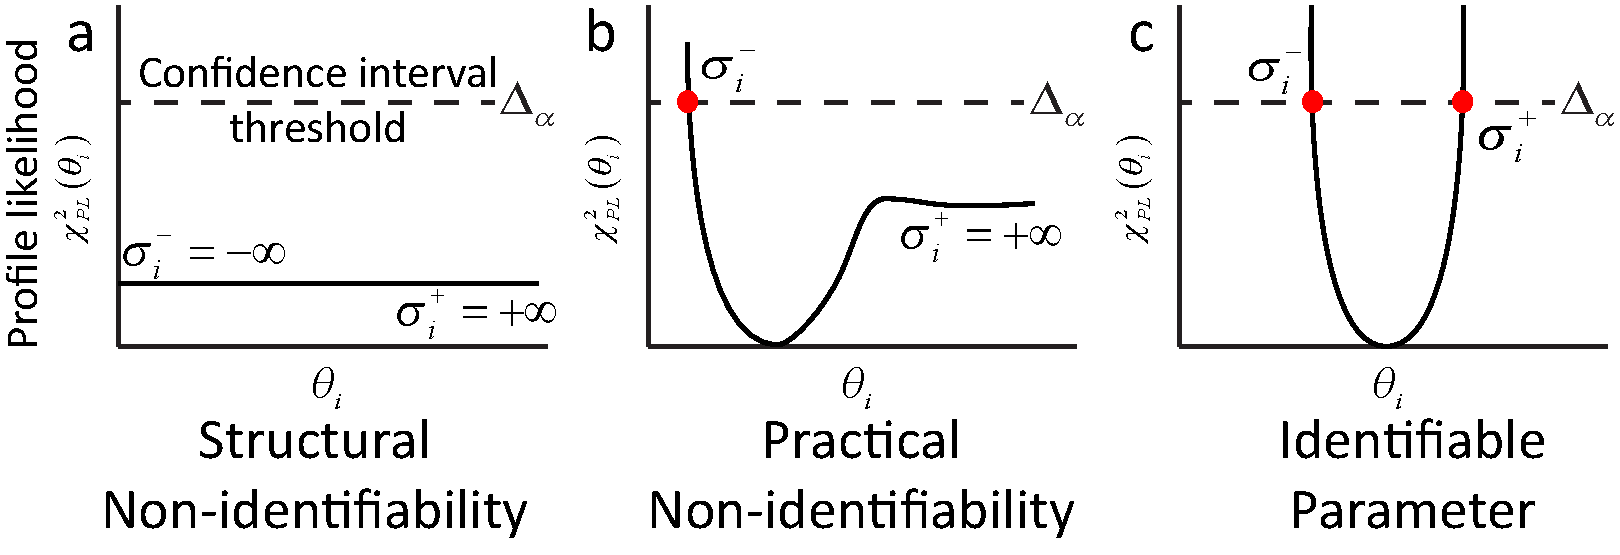
\includegraphics[width=.8\textwidth,height=.8\textheight,keepaspectratio]{figures/identifiability}}
		\caption{The profile likelihood estimates of a) a structurally non-identifiable, b) a practically non-identifiable and c) an identifiable parameter. The horizontal axis represents the changes in the value of the parameter ($\theta_i$) whose identifiability is being determined and the profile likelihood ($\chi^2_{PL}(\theta_i)$) is shown in the vertical axis. The confidence interval threshold ($\Delta_{\alpha}$) used to determine the identifiability of the parameter is denoted by the horizontal dotted line. Identifiable parameters are distinguished from non-identifiable parameters by the presence of both upper and lower bounds on their confidence interval estimates $\left[\sigma_{i}^-,\sigma_{i}^+\right]$. }\label{fig:identtypes}
	\end{figure}	
	
	Due to the dependence of practical parameter identifiability on the experimental data, the profile likelihood approach can be used to design experiments in such a way that the observables that are derived from these experiments can improve the practical identifiability of the parameters. We show how experimental design can have a meaningful impact on parameter identification and estimation in Figure \ref{fig:edwithpl}.	Assuming a parameter $\theta_i$ is practically non-identifiable (Figure \ref{fig:edwithpl}a), performing a profile-likelihood based identifiability analysis using simulated data can help determine the nature of experiments needed to make the parameter identifiable (Figure \ref{fig:edwithpl}b). In contrast, performing non-informative experiments without prior knowledge on their ability to change the identifiability of the parameter may provide data that cannot be used to estimate parameter $\theta_i$ (Figure \ref{fig:edwithpl}c).	
	
	\subsection{A method to establish posterior identifiability of metabolic network models:}
	This section details a method to establish the practical (posterior) identifiability of metabolic network models using the algebraic relationship between fluxes.
	Every flux, $v$, in a kinetic model of a metabolic network can be expressed as a nonlinear algebraic equation (Equation \ref{eq:flux_gen}). The fluxes are expressed as a function of the metabolite concentrations $x$ and the kinetic parameters $\theta$ in Equation (\ref{eq:flux_gen}).
	\begin{align}\label{eq:flux_gen}
		v = f(\mathbf{x},\mathbf{\theta})
	\end{align}
	Given the nonlinear nature of this model, the function $f$ in Equation (\ref{eq:flux_gen}) can expressed, without loss of generality as,
	\begin{align}\label{eq:nr_dr}
		v = \frac{N(\mathbf{x},\theta)}{D(\mathbf{x},\theta)}
	\end{align}
	where $N(\mathbf{x},\theta)$ is the numerator of $f$, and $D(\mathbf{x},\theta)$ is the denominator of $f$.
	
	If $\theta \in \mathbb{R}^p$, given a set of experimental measurements for the metabolite concentrations $\mathbf{x}$ and the reaction fluxes $\mathbf{v}$, theoretically, it is possible to choose $p$ sets of data from these measurements to solve for the $p$ parameters in $\theta$. However, if any these datasets do not satisfy the condition that $D(\mathbf{x},\theta) \neq 0$, then the number of experiments required to estimate the $p$ parameters in $\theta$ can be established to be greater than $p$. An example is shown below.
	
	This analysis can be performed for each flux in a metabolic network independent of all the other fluxes. This enables this method to be scalable to even genome-scale models. The following section demonstrates this methodology for one of the fluxes in the gluconeogenic model of Kotte et al., \parencite{Kotte2014}.
		
	\subsection{Identifiability analysis of parameters in a kinetic model of gluconeogenesis:}
	The proposed model for acetate consumption through gluconeogenesis and its corresponding kinetic model is used as a case study to illustrate the utility of identifiability analysis for the design of experiments for estimating parameters in kinetic models of metabolism. The kinetic model is described below.
	\begin{equation}\label{eq:ode1}
	\frac{d}{dt}pep=v_1-v_2-v_4
	\end{equation}
	\begin{equation}\label{eq:ode2}
	\frac{d}{dt}fdp=v_2-v_3
	\end{equation}
	\begin{equation}\label{eq:ode3}
	\frac{d}{dt}E=v_{e,max}\left(\frac{1}{1+\left(\frac{fdp}{K_{e}^{fdp}}\right)^{n_e}}\right) - d E
	\end{equation}
	The kinetic expressions for fluxes $v_1$ through $v_4$ are given below. The consumption of acetate through $v_1$ and conversion of \textit{pep} through $v_2$ are expressed in Equations (\ref{eq:flux1}) and (\ref{eq:flux2}) respectively using Michaelis-Menten kinetics. The acetate flux through $v_1$ is also governed by the quantity of available enzyme E. 
	\begin{equation}\label{eq:flux1}
	v_1 = k_{1}^{cat}E\frac{acetate}{acetate+K_{1}^{acetate}}
	\end{equation}	
	\begin{equation}\label{eq:flux2}
	v_2 = V_{2}^{max}\frac{pep}{pep+K_{2}^{pep}}
	\end{equation}
	\begin{equation}\label{eq:flux3}
	v_3 = V_{3}^{max}\frac{\tilde{fdp}\left(1+\tilde{fdp}\right)^3}{\left(1+\tilde{fdp}\right)^4+L_3\left(1+\frac{pep}{K_{3}^{pep}}\right)^{-4}}
	\end{equation}
	The allosterically regulated flux $v_3$ for the consumption of \textit{fdp} is expressed in Equation (\ref{eq:flux3}) using the Monod-Wyman-Changeux (MWC) model for allosterically regulated enzymes, where $\tilde{fdp}$ refers to the ratio of \textit{fdp} with respect to its allosteric binding constant $K_{3}^{fdp}$. The added flux $v_4$ for the export of \textit{pep} is expressed as a linear equation dependent on $pep$ in Equation (\ref{eq:flux4}).
	\begin{equation}\label{eq:flux4}
	v_4 = k_{4}^{cat}.pep
	\end{equation}
	
	We use flux $v_2$ to demonstrate the identifiability analysis method described in the previous section. Flux $v_2$ has two parameters, $V_2^{max}$ and $K_2^{pep}$ that need to be estimated from experimental data. Here, we assume that at least two different sets of experimental data for the concentrations and fluxes are available. Accordingly, we label these dataset as ${pep}^1$, ${v_2}^1$ and ${pep}^2$, ${v_2}^2$ respectively. Subsequently, these experimental datasets can be included in the model to form two simultaneous nonlinear algebraic equations in the parameters $V_2^{max}$ and $K_2^{pep}$ (Equation \ref{eq:v2_par}).
	
	\begin{subequations}\label{eq:v2_par}
		\begin{align}		
		V_2^{max} = \frac{v_2^1v_2^2(pep^1-pep^2)}{v_2^2pep^1-v_2^1pep^2}\\
		K_2^{pep} = \frac{pep^1(v_2^1pep^2-v_2^2pep^2)}{v_2^2pep^1-v_2^1pep^2}
		\end{align}
	\end{subequations}
	
	\begin{table}[!tbhp]
		\caption{Table showing the perturbed values of all fluxes used for parameter estimation.}
		\begin{center}				
			\begin{tabular}{ccc}
				Designation & Perturbed Fluxes & Perturbed Values\\
				\hline
				P1 & $v_1$ & 2\\
				P2 & $v_2$ & 0.2\\
				P3 & $v_3$ & 0.5
			\end{tabular}
		\end{center}	
		\label{tab:pval}
	\end{table}

	\section{Results:}
	\paragraph{Outline:}
	\begin{itemize}
		\item parameter estimation is a well developed field typically using minimization of least square error to estimate model parameters from available experimental data
		\item if parameters are structurally identifiable, it does not guarantee practical identifiability from noisy experimental data
		\item identifiability dependent on whether given datasets (outputs) for estimation can sufficiently distinguish between different parameter values
	\end{itemize}
	
	\paragraph{Sections:}
	\begin{itemize}
		\item datasets required for parameter estimation in kinetic models of metabolism (methods?)		
		\item identifiability in kotte model - scalability, number of experiments required, requirements for time course data(? in the intro)		
		\item identifiability in large rbc model
	\end{itemize}
	
	\printbibliography
\end{document}